
Ons GPU is ingedeeld volgens het volgende blokschema.
\begin{figure}[H]
\centering
        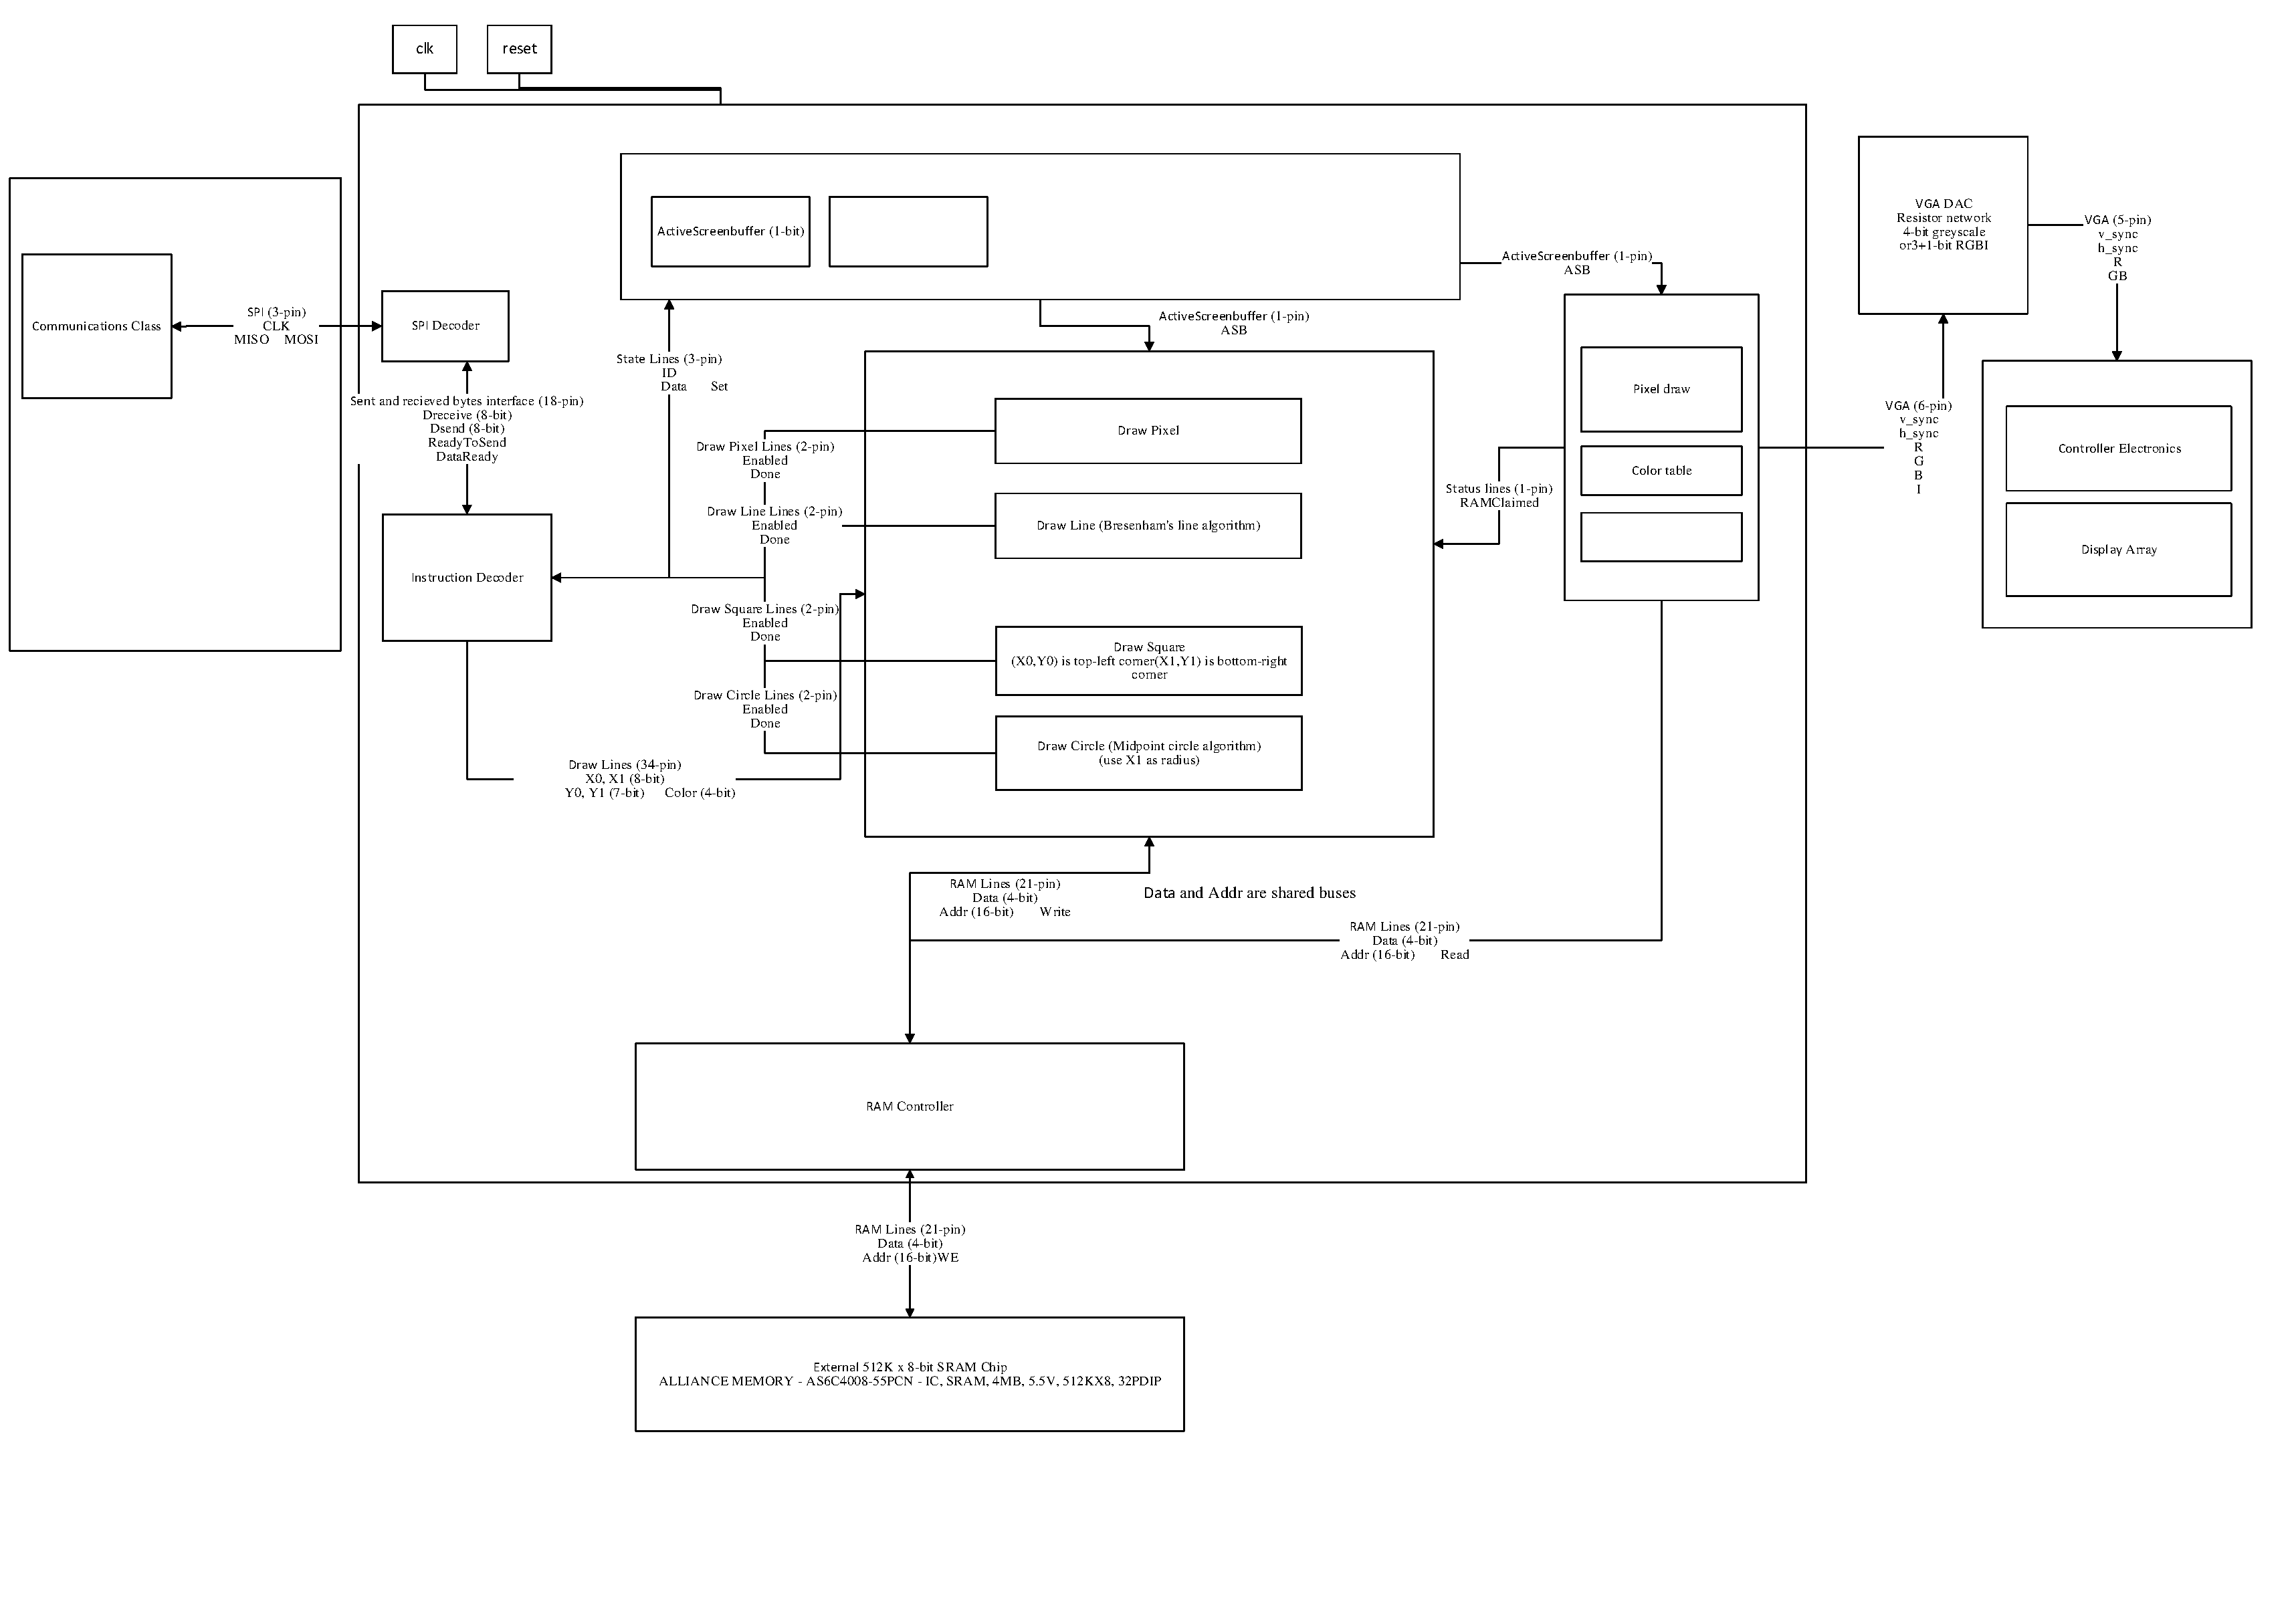
\includegraphics[width=\linewidth]{inputfiles/systeemdrawing-rc.pdf}
        \caption{Blokschema GPU}
        \label{fig:Blokschema GPU}
\end{figure}


\subsection{SPI Controller}
Voor de communicatie tussen de arduino en onze GPU hebben we een SPI decoder nodig. De ingang SS staat voor slave select, dit wordt normaal gebruikt voor het geval dat je meerdere slave chips hebt, aangezien dit bij ons niet het geval is zal dit signaal altijd hoog zijn. Het signaal SCLK is voor het CLK signaal voor de communicatie. Als laatste ingang is er de MOSI, dit staat voor master out en slave in, dit is de daadwerkelijke data die verzonden wordt van de arduïno naar onze gpu. Voor de uitgangen hebben we MISO, master in slave out, dit is om de volgende instructie aan te vragen van de arduïno. Dan zijn er nog de uitgangen naar de instructie decoder, de 8 bits data bus voor om alle data te sturen als de data ready hoog is.

\begin {itemize}
\item ingangen:
\begin {itemize}
\item MOSI 
\item SS (1 bit altijd hoog)
\item SCLK (clk signaal)
\item readytosend (1 bit)
\end {itemize}
\item uitgangen:
\begin {itemize}
\item MISO
\item 8 bits data bus
\item data ready
\end {itemize}
\end {itemize}

\subsection{Instruction Decoder}
De instructiedecoder zorgt ervoor dat de data, die vanuit de arduino komt, vertaald wordt in data (instructies), waar verschillende onderdelen van de gpu mee over weg kunnen. 
Dit houdt in dat de intructiedecoder het draw-blok van de juiste informatie voorziet, zodat deze bijvoorbeeld pixels kan tekenen die in het stateregister opslagen worden om in de screenbuffer geschreven te worden.
De instructiedecoder heeft (op dit moment) een 8-bits bus ingang van de SPI decoder, deze wordt ingelezen als de ingang data ready hoog is.
Wanneer dan een complete instructie, van minimal één keer 8 bits, verstuurd is, zal er een signaal worden gegeven dat de volgende instructie kan worden gestuurd.
Als uitgangen van de instructiedecoder zijn er de coördinaten van het te tekenen object met de kleur die dit object moet hebben, deze signalen gaan natuurlijk naar het draw-blok.
Om de juiste module van het draw-blok aan te sturen wordt gebruik gemaakt van een enabled signaal dat aangeeft welke module de instructie moet uitvoeren.
Van het draw-blok krijgt de instructiedecoder een signaal als het klaar is met tekenen zodat deze weer een volgend object kan tekenen. 
Verder wordt de instructiedecoder gebruikt om te bepalen welk screenbuffer er gebruikt wordt om op te schrijven en dus indirect welke om te lezen. Deze informatie wordt verstuurd naar een stateregister doormiddel van een signaal set en de data voor de juiste screenbuffer. Dit alles wordt gedaan synchroon met de klok.

\begin {itemize}
\item Ingangen:
\begin{itemize}
\item clk (clock, std\_logic)
\item reset (std\_logic)
\item di (data in, std\_logic\_vector)
\item dav (data available, std\_logic)
\item draw\_rdy (instruction processed, std\_logic)
\end{itemize}

\item Uitgangen:
\begin{itemize}
\item rts (ready to send, read do, std\_logic)
\item do (data out, 00000110 when instruction processed, std\_logic\_vector).
\item color (std\_logic\_vector)
\item x0 (std\_logic\_vector)
\item y0 (std\_logic\_vector)
\item x1 (std\_logic\_vector)
\item y1 (std\_logic\_vector)
\item en (draw-block selector, std\_logic\_vector)
\item reg\_id (register selector, std\_logic (wellicht uitgebreid naar vector wanneer meer dan twee registers benodigd zijn))
\item reg\_set (register set, std\_logic)
\item reg\_value (register value (current screen buffer), std\_logic)
\end{itemize}
\end{itemize}

\subsection{Draw Logic}
In dit blok worden de instructie omgezet naar pixels, vierkanten, lijnen, cirkels en eventueel meer. Dit blok krijgt de informatie binnen van de instructiedecoder, deze geeft aan welke module er gebruikt moet worden met de bijbehorende coördinaten en kleur.
De keuze voor welke module er gebruikt moet worden gebeurd doormiddel van het signaal enabled. Verder neemt het draw blok het signaal ASB mee, zodat er in de juiste screenbuffer geschreven wordt. Tevens krijgt het draw-blok het signaal RAMclaimed binnen van de VGA controller, dit houdt in dat als de VGA controller aan het lezen is in het RAM dat het draw-blok er niet in kan schrijven. Als laatste ingang krijgt het draw-blok een signaal write binnen van de RAM controller dat zegt wanneer er geschreven mag worden.
Als uitgangen heeft het draw-blok het signaal done als de module klaar is met het tekenen van een de instructie zodat er een volgende instructie kan doorgegeven worden. Verder heeft het de uitgangen naar de RAM controller, hierin worden de kleur 

\begin {itemize}
\item ingangen:
\begin {itemize}
\item kleur (4 bits)
\item x coördinaat (8 bits)
\item y coördinaat (7 bits)
\item enabled (1 bit)
\item ASB (1 bit)
\item RAMclaimed (1 bit)
\item write (1 bit)
\end {itemize}

\item uitgangen:
\begin {itemize}
\item kleur (4 bits)
\item adres (16 bits)
\item done (1 bit)
\end {itemize}
\end{itemize}

\subsubsection { pixel}
Hierin worden aparte pixels getekend, hiervoor zijn de x,y coördinaten en de kleur nodig.

\subsubsection { square}
In deze module wordt een vierkant getekend met de x,y coördinaten van de eerste pixel links boven en de laatste pixel rechtsonder van het vierkant en natuurlijk de kleur die het vierkant moet hebben.

\subsubsection { lijn}
Hier wordt het algoritme van Bresenham gebruikt hiervoor hebben we de x,y coördinaten nodig van het begin en het eindpunt van de lijn.

\subsubsection { cirkel}
In deze laatste module gebruiken we het midpoint circle algoritme met x1 als de radius.

\subsection{RAM Controller}
Omdat we een externe RAM gebruiken voor onze screenbuffers is het nodig om hiervoor communicatie op te stellen, zodat er in het juiste gedeelte van de RAM geschreven en gelezen wordt en dat dit niet tegelijkertijd gebeurd, omdat het RAM dat niet aankan. We hebben voor een externe RAM gekozen omdat er geen RAM geheugen groot genoeg gemaakt kon worden met de benodigde transistoren om bijvoorbeeld de screenbuffers te renderen. De RAM controller stuurt naar het draw-blok een signaal write als het mag gaan schrijven in het RAM geheugen, de RAM controller krijgt dan de kleur en het adress binnen van het draw-blok. Als de VGA controller mag gaan lezen krijgt het een signaal read binnen van de RAM controller dan zal er weer data naar de VGA controller verstuurd worden, kleur en adres.

\begin {itemize}
\item ingangen:
\begin {itemize}
\item kleur (4 bits)
\item adres (16 bits)
\end {itemize}
\item uitgangen:
\begin {itemize}
\item write (1 bit)
\item read (1 bit)
\item kleur (4 bits)
\item adres (16 bits)
\end {itemize}
\end {itemize}

\subsection{VGA Controller}
De VGA controller is er om de screenbuffer uit te lezen en de data die daarin staat naar het beeldscherm te sturen. Het leest van de screenbuffer op het moment dat er niet in geschreven wordt, de inverse van ASB dus. Als de controller het RAM geheugen claimt met het signaal RAMclaimed mag er niet worden geschreven in het RAM. De VGA controller leest dan de signalen h- en v-sync (de positie van de pixel) en de waardes van RGBI ( rood , groen, blauw en de intensiteit) af. Het uitlezen van de screenbuffer kost 55 ns en is dus snel genoeg aangezien een klokpuls 160 ns is. In de overige tijd kan er dus geschreven worden in het RAM.

\begin {itemize}
\item ingangen:
\begin {itemize}
\item active screen buffer (1 bit)
\item read (1 bit)
\item kleur (4 bits)
\item adres (16 bits)
\end {itemize}
\item uitgangen:
\begin {itemize}
\item RAMclaimed (1 bit)
\item hsync (1 pin)
\item vsync (1 pin)
\item RGBI (4 pinnen)
\end {itemize}
\end {itemize}
